\chapter{Kriptografi}
Ada dua cara untuk mengamankan data, yaitu menyembunyikan data atau menyandikan
data. Cara pertama menggunakan steganografi, sementara cara kedua menggunakan
kriptografi. Bab ini akan membahas lebih banyak tentang kriptografi, meskipun
steganografi akan disinggung secara singkat.

Ilmu ini pada awalnya dianggap terlarang untuk diajarkan sehingga tidak ada
bahan bacaan untuk mempelajarinya. Setelah David Kahn membuat bukunya di tahun
1969, maka ilmu pengamanan data ini menjadi lebih terbuka untuk dipelajari.
Saat ini sudah sangat banyak buku yang membahas mengenai hal ini, mulai dari
yang umum~\cite{levycrypto} (tidak teknis) sampai ke yang teknis.


\section{Steganografi}
Steganografi ({\em steganography}) adalah ilmu untuk menyembunyikan pesan
sehingga tidak terlihat dengan mudah. Mekanisme penyembunyian ({\em hide}, {\em
concealment}) dilakukan dengan menggunakan media lain. Sebagai contoh, kita
dapat menyembunyikan pesan dalam gambar ({\em image}, foto), audio, atau video.
Dalam sejarahnya, penyembunyian pesan dapat dilakukan dengan menggunakan meja
yang dilapisi lilin (jaman perang antara Yunani dan Persia).

Saat ini steganografi digunakan sebagai bagian dari {\em Digital Rights
Management} (DRM), misalnya dengan menyisipkan informasi mengenai HaKI dari
produk digital (musik, ebook, foto, dan sejenisnya).

\begin{figure}[ht]
\fbox{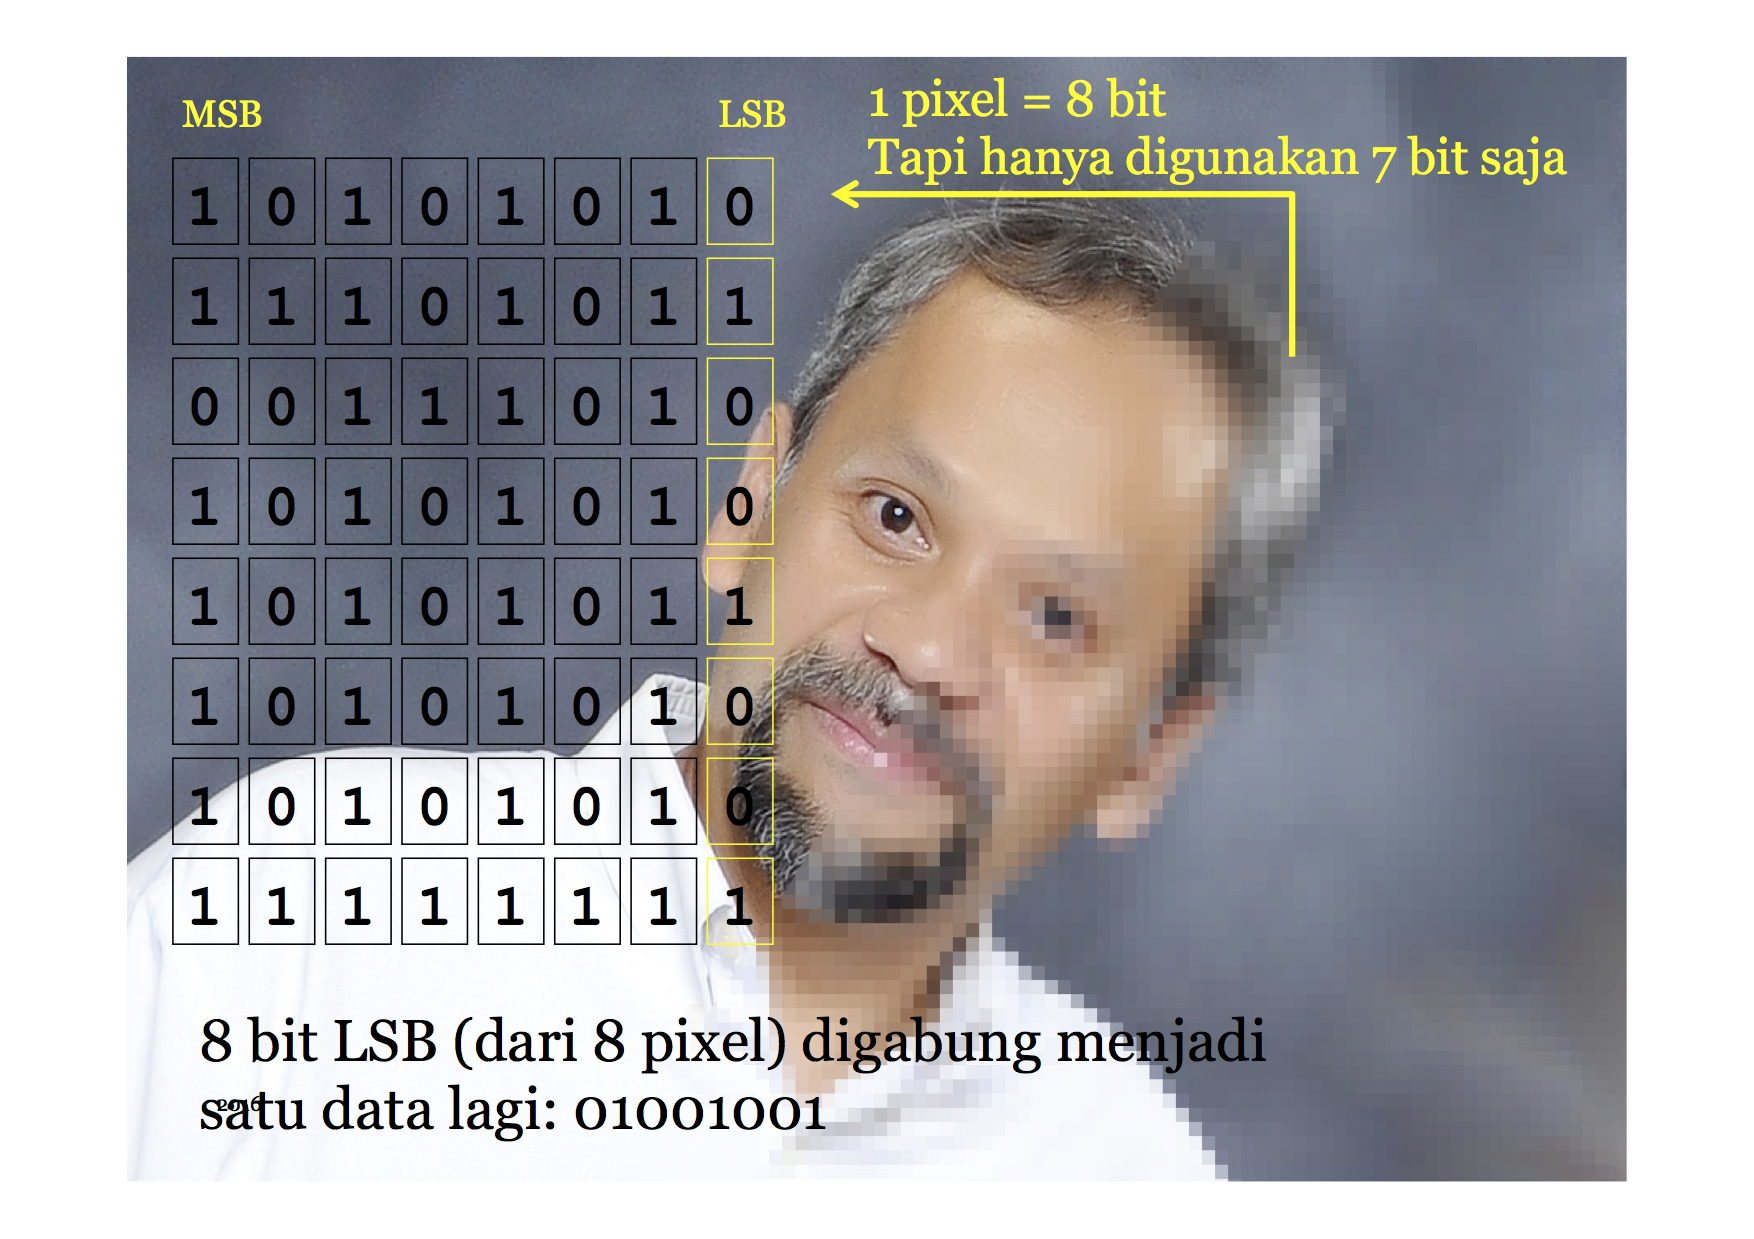
\includegraphics[width=1.0\linewidth]{graphics/BR-watermark.png}}
\caption{Contoh Watermark}
\label{fig:watermark}
\end{figure}

Ada banyak cara untuk menyisipkan informasi ke dalam berkas digital. Sebagai
contoh, kita dapat menyisipkan pesan di dalam gambar (foto) digital seperti
ditampilkan pada Gambar~\ref{fig:watermark}. Cara yang digunakan adalah
dengan menggunakan {\em least significant bit} (LSB) dari data {\em pixel}
gambar. Misalnya, sebuah {\em pixel} (titik) di gambar direpresentasikan oleh
8-bit. Dalam hal ini ada 256 kombinasi (katakanlah skala abu-abu / grey scale).
Maka kita dapat mengorbankan bit yang ke-8 tersebut dan hanya menggunakan 7-bit
saja dalam pewarnaan. Bit ke-8 dapat kita gunakan sebagai bagian dari data.
Jika ada 8 bit yang berurutan kita perlakukan seperti itu, maka akan ada tempat
untuk 8-bit data (1 byte). Jika ini kita teruskan lagi, maka kita dapat
menyimpan beberapa (banyak) bytes di dalam gambar itu.
Data yang kita simpan di dalam berkas (gambar) tersebut dapat berupa
kepemilikan gambar, {\em copyright}, misalnya. 

Tentu saja contoh di atas agak sedikit menyederhanakan permasalahan.
Steganografi yang bagus akan tahan bantingan terhadap proses-proses tertentu.
Sebagai contoh, jika gambar tersebut diubah ukurannya ({\em resize}) maka
informasi yang ditanamkan tersebut akan hilang. Algoritma steganografi yang
bagus akan memiliki kekuatan yang lebih dari itu.


\section{Kriptografi}
Berbeda dengan steganografi, kriptografi tidak menyembunyikan pesan tetapi
mengubah pesan sehingga sulit diperoleh pesan aslinya. Pesan diubah dengan cara
{\bf transposisi} (mengubah letak dari huruf) dan {\bf substitusi} (mengganti
huruf/kata dengan huruf/kata lainnya). Pesan yang sudah diubah terlihat seperti
sampah, tetapi tetap terlihat oleh penyerang atau orang yang tidak berhak.

Proses transposisi dapat dilakukan dengan berbagai cara. Sebagai contoh, kita
dapat menulis pesan menjadi dua baris secara bergantian. Huruf pertama
diletakkan di baris pertama, huruf kedua di baris kedua, huruf ketiga di baris
pertama lagi, huruf keempat di baris kedua lagi, dan seterusnya. Mari kita
ambil contoh kalimat ``selamat datang di kota bandung''. Kalimat ini akan kita
tuliskan secara bergantian. (Dalam contoh ini, spasi kita buang saja.)

\begin{mdframed}
\begin{verbatim}
slmtaagioaadn
eaadtndktbnug
\end{verbatim}
\end{mdframed}

Kalimat yang akan dikirimkan menjadi ``slmtaagioaadneaadtndktbnug''. Kalimat
ini yang kita kirimkan. Dapat dilihat bahwa kalimat yang dikirimkan sudah sulit
dibaca isinya. Di sisi penerima akan dilakukan proses sebaliknya sehingga
didapat kalimat aslinya.


Secara umum ada tiga komponen utama dari kriptografi, yaitu {\em plain text},
{\em ciphertext}, dan algoritma serta kunci yang digunakan\footnote{Pada
awalnya, kunci melekat dengan algoritma. Namun kemudian, kunci dipisahkan dari
algoritma. Kekuatan dari sebuah sistem kriptografi bergantung kepada
kerahasiaan dari kuncinya, bukan dari kerahasiaan algoritmanya.}.
\begin{itemize}
  \item {\em Plain text} adalah data (teks, pesan, {\em message}) asli yang
  belum diproses. Meskipun disebut plain text, sesungguhnya data asli tidak
  harus berupa teks (ASCII). Plain text dapat juga berupa berkas biner.
  \item {\em Ciphertext} adalah data yang dihasilkan dari proses enkripsi.
     {\em Ciphertext} dapat berbentuk berkas biner atau ASCII. Perlu diasumsikan
  bahwa penyerang kemungkinan dapat mengakses ciphered text.
  \item Algoritma dan kunci merupakan {\em black box} yang memproses plain text
  menjadi ciphered text. Algoritma diasumsikan diketahui oleh penyerang,
  tetapi kunci tidak diketahui.
\end{itemize}

Hubungan antara ketiga komponen tersebut dapat dirumuskan sebagai berikut.
{\em Ciphertext} $c$ merupakan hasil operasi enkripsi ({\em encryption}) $E$ 
dengan kunci $k$ terhadap pesan $m$. {\em Ciphertext} ini yang nanti dikirimkan
kepada pihak yang dituju.

\begin{equation}
   c = E_k(m)
\end{equation}

Di sisi sebaliknya, yaitu di sisi penerima, pesan ({\em plain text}) $m$
diperoleh dari hasil proses dekripsi ({\em decryption}) $D$ dengan kunci $k$
terhadap {\em ciphertext} $c$.

\begin{equation}
   m = D_k(c)
\end{equation}

Jika kita menggunakan algoritma kriptografi kunci privat, yang akan dibahas
kemudian, kunci ($k$) yang sama digunakan untuk proses enkripsi dan dekripsi.
Untuk algoritma kriptografi yang berbasis kunci public, kunci yang digunakan
untuk proses enkripsi dan dekripsi berbeda.


\subsection{Kriptografi Kunci Privat}
Kriptografi kunci privat adalah jenis kriptografi yang paling banyak dikenal.
Pada sistem kriptografi ini, ada satu kunci yang digunakan untuk mengunci dan
membuka. Itulah sebabnya sistem ini dikenal juga dengan istilah kriptografi
{\bf simetrik}. Kunci yang digunakan harus dirahasiakan sehingga kriptografi
ini disebut kriptografi kunci privat.

Ada banyak algoritma yang mengimplementasikan kriptografi kunci privat, antara
lain DES, Blowfish, dan AES. (Penjelasan rinci mengenai algoritma-algoritma ini
akan dibahas secara terpisah.) Algoritma-algoritma ini umumnya sangat cepat
dalam operasinya.

Salah satu kesulitan dari pengoperasian sistem kriptografi kunci privat adalah
dalam hal distribusi kunci ({\em key distribution}). Sebagai contoh, jika {\em
Alice} ingin mengirim pesan kepada {\em Bob}, maka mereka berdua memiliki
sebuah kunci yang sama. Jika {\em Alice} ingin mengirim pesan ke orang lain,
katakan {\em Charlie}, maka mereka berdua memiliki kunci sendiri ({\em
Alice-Charlie}) yang berbeda dengan kunci {\em Alice-Bob}. Demikian pula jika
{\em Bob} dan {\em Charlie} ingin berkomunikasi maka mereka memiliki kunci
sendiri ({\em Bob-Charlie}). Jika kita teruskan dengan pihak-pihak lain, maka
jumlah kunci yang dibutuhkan akan meledak secara eksponensial sesuai dengan
penambahan jumlah pengguna ($n$).

\begin{equation}
   numkeys = \frac{(n) (n-1)}{2}
\end{equation}

Untuk jumlah pengguna yang sedikit, misal puluhan orang, maka jumlah kunci yang
beredar tidak terlalu banyak. Begitu jumlah pengguna sangat banyak, maka jumlah
kunci menjadi sangat besar seperti dapat dilihat pada
tabel~\ref{tbl:jumlahkunci}. Bayangkan jumlah pengguna internet di dunia ini.
Berapa banyak kunci yang harus dipersiapkan jika semuanya akan saling
berkomunikasi satu dengan lainnya?

\begin{table}
   \centering
   \caption{Jumlah Kunci}
   \label{tbl:jumlahkunci}
\begin{tabular}{ r r }
   $n$ & Jumlah kunci \\
   \hline
  10 & 45 \\
  100 & 4.950 \\
  1000 & 499.500 \\
  10.000 & 49.995.000 \\
  100.000 & 4.999.950.000 \\
\end{tabular}
\end{table}

Meskipun ada masalah distribusi kunci, sistem kriptografi kunci privat ini yang
paling baik kinerjanya (performance) sehingga dia sangat dibutuhkan.


\subsection{Kriptografi Kunci Publik}
Pada sistem kriptografi kunci publik, ada dua kunci yang akan digunakan. Setiap
pelaku akan memiliki sepasang kunci ({\bf kunci publik} dan {\bf kunci privat})
yang saling berhubungan. Jika sebuah pesan dikunci dengan kunci publik, maka
dia hanya dapat dibuka oleh kunci privat pasangannya. Demikian pula jika sebuah
pesan dikunci oleh kunci privat, maka dia hanya dapat dibuka oleh kunci publik
pasangannya. (Jangan bingung. Baca berulang kali. Nanti akan dijelaskan dengan
cara lain lagi.)

Sistem ini sering juga disebut {\bf kriptografi asimetrik}, karena kunci yang
dipakai untuk mengunci berbeda dengan kunci untuk membuka. Asimetrik.

Sesuai dengan namanya, kunci publik boleh diketahui oleh umum dan disimpan di
tempat publik. Sementara itu, kunci privat hanya boleh diakses oleh pemiliknya.
Selama-lamanya kunci privat ini tidak boleh terbuka. Jika kunci privat ini
tercuri, maka identitas kita juga tercuri.
